\chapter{The \glsentrytext{holoassist} API}\label{appendix:external_meshes_api}

All the previous chapters focus on the inner workings of \gls{holoassist}, but gloss over the exact technicalities of how its \gls{API} works, as they can be seen as implementation details. These details are available here, and this section constitutes the documentation for the currently available \gls{API}.

\Gls{holoassist} uses an \gls{UDP}-based \gls{API}: each packet is an individual \gls{API} command which, when received, triggers a certain action. Each packet contains a string that consists of a single, serialized JSON\cite{bray_javascript_2017} object. This JSON object always contains a \texttt{type} field, which identifies what action it will trigger in \gls{holoassist}. The other fields differ across different types of commands. The commands can be split in two big groups: those that act on \glspl{geofixedaug} and those that instead target \glspl{planefixedaug}. These groups are described in the following sections.

The last part of \gls{holoassist}'s \gls{API} is the way in which simulator status updates are dispatched to it, which however has already been described in details in \autoref{sec:renderling_elm} (in particular \autoref{table:sim_status_update_udp_packet}).

\section{Commands for \glsentrytext{geofixedaug}}

Displaying a \gls{geofixedaug} entails creating a \gls{gfelm} and creating its vertices and indices. These changes are not applied immediately to what is shown to the user, but need to be committed first with a dedicated command: this allows to partially/slowly update the mesh without disrupting the user experience and then, when all the updates are done, immediately show the new desired result. Creating a new \gls{gfelm} can be done with the JSON message shown in \autoref{lst:gf_create_elm}. After creation, vertices can be added or modified with the JSON message shown in \autoref{lst:gf_set_vertices}. Indices can be handled in a similar way, shown in \autoref{lst:gf_set_indices}. There currently is no way of deleting already submitted vertices or indices, as that would make the whole \gls{API} significantly more complicated (e.g. what should happen to the index list if some of the referenced vertices are deleted?). When the list of vertices and indices is complete, the changes can be committed with the command shown in \autoref{lst:gf_commit}: only at this point, the mesh shown to the user is actually updated. Before being able to see something, a last step is needed: the mesh needs to be activated with the command shown in \autoref{lst:gf_activate}. The activation status of a \gls{gfelm} can be toggled to temporarily hide it from the user's sight without deleting it, and by default a newly created mesh is deactivated. Finally, when a mesh is not needed anymore, it can be deleted with the command shown in \autoref{lst:gf_delete}.

\begin{figure}
  \centering
  \begin{tabular}{c}
  \begin{lstlisting}[language=json]
    {
        "type": "CREATE_MESH",
        "id": "example_mesh_id",
        "interpolateOnCommit": true,
        "interpolatedSegmentMaxLengthMeters": 50
    }
  \end{lstlisting}
  \end{tabular}
  \caption{Creates a new \gls{gfelm}. The \texttt{id} field is used to identify the created mesh in subsequent commands and the other two fields allow control over the automatic interpolation mesh interpolation described in \autoref{sec:automatic_interpolation}.}\label{lst:gf_create_elm}
\end{figure}

\begin{figure}
  \centering
  \begin{tabular}{c}
  \begin{lstlisting}[language=json]
    {
        "type": "SET_MESH_VERTICES",
        "id": "example_mesh_id",
        "startIndex": null,
        "vertices": [{
            "originWgs": {
                "latitudeRadians": 0.844094,
                "longitudeRadians": 0.205382,
                "altitudeMeters": 453
            },
            "color": [0.0, 1.0, 0.0, 1.0],
            "localPositionMeters": [0, 0, 0],
            "localRotationRadians": [0, 0, 0]
        }]
    }
  \end{lstlisting}
  \end{tabular}
  \caption{Adds or modifies a list of \texttt{GeoFixedVertex}. The \texttt{id} field specifies which mesh will be modified by this command. \texttt{startIndex} can be either \texttt{null}, in which case the vertices will be added at the end of the current list, or an integer indicating a zero-based index $i$ inside the current list of vertices, in which case this command will replace the \emph{already existing} vertices of the mesh starting from $i$ until all the vertices contained in the command are processed. In this second case, no new vertices will be created. The field \texttt{vertices} represents a list of \texttt{GeoFixedVertex}: the details of such structure are available in \autoref{sec:geofixedaug_representation}. \texttt{originWgs} describes the topocentric origin of the vertex.}\label{lst:gf_set_vertices}
\end{figure}

\begin{figure}
  \centering
  \begin{tabular}{c}
  \begin{lstlisting}[language=json]
    {
        "type": "SET_MESH_INDICES",
        "id": "example_mesh_id",
        "startIndex": null,
        "indices": [1, 2, 2, 3]
    }
  \end{lstlisting}
  \end{tabular}
  \caption{Extends or modifies the list of indices of an \gls{gfelm}. The \texttt{id} field specifies which mesh will be modified by this command. \texttt{startIndex} can be either \texttt{null}, in which case the indices will be added at the end of the current list, or and integer indicating a zero-based index $i$ inside the current list of indices, in which case this command will replace the \emph{already existing} indices of the mesh starting from $i$ until all the indices contained in the command are processed. In this second case, no new indices will be created. The field \texttt{indices} consists of a list of integers, each of which will become an element in the list of indices and is the index of a vertex in this mesh's vertex list. The list of indices must contain an even amount of indices, as each pair denotes a line.}\label{lst:gf_set_indices}
\end{figure}

\begin{figure}
  \centering
  \begin{tabular}{c}
  \begin{lstlisting}[language=json]
    {
        "type": "COMMIT_MESH_CHANGES",
        "id": "example_mesh_id"
    }
  \end{lstlisting}
  \end{tabular}
  \caption{Commits the changes and displays them to the user. The \texttt{id} field is used to identify the mesh whose changes should be committed.}\label{lst:gf_commit}
\end{figure}

\begin{figure}
  \centering
  \begin{tabular}{c}
  \begin{lstlisting}[language=json]
    {
        "type": "SET_MESH_ACTIVE",
        "id": "example_mesh_id",
        "active": true
    }
  \end{lstlisting}
  \end{tabular}
  \caption{Changes the activation status of a \gls{gfelm}. The \texttt{id} field is used to identify which mesh should be edited and the \texttt{active} field specifies whether the mesh should be activated or deactivated.}\label{lst:gf_activate}
\end{figure}

\begin{figure}
  \centering
  \begin{tabular}{c}
  \begin{lstlisting}[language=json]
    {
        "type": "DELETE_MESH",
        "id": "example_mesh_id"
    }
  \end{lstlisting}
  \end{tabular}
  \caption{Completely deletes a \gls{gfelm}. The \texttt{id} field is used to identify which mesh should be deleted.}\label{lst:gf_delete}
\end{figure}

\section{Commands for \glsentrytext{planefixedaug}}

Commands for \glspl{planefixedaug} are very similar to those for \glspl{geofixedaug}, with just a few differences:

\begin{enumerate}
    \item The \texttt{type} of each command is prefixed with \texttt{PF\_}, to clearly distinguish which kind of meshes are being manipulated. For example, \texttt{CREATE\_MESH} becomes \texttt{PF\_CREATE\_MESH}. Except for what is listed below, the remaining part of the JSON message remains unchanged.
    \item When creating a mesh, the parameters regarding the interpolation are replaced with fields specifying the pose of the \gls{planefixedaug} in the airplane mesh coordinate system, as shown in \autoref{lst:pf_create_mesh}.
    \item The \texttt{vertices} field of a \texttt{PF\_SET\_MESH\_VERTICES} command is a list of objects like the one shown in \autoref{lst:pf_vertex}, and not of \texttt{GeoFixedVertices}.
\end{enumerate}

Moreover, an additional command to change the position and rotation of the mesh is available, as shown in \autoref{lst:pf_update}.

\begin{figure}
  \centering
  \begin{tabular}{c}
  \begin{lstlisting}[language=json]
    {
        "type": "PF_CREATE_MESH",
        "id": "example_mesh_id",
        "originPositionMeters": [0.0, 0.0, 0.0],
        "originRotationRadians": [0.0, 0.0, 0.0]
    }
  \end{lstlisting}
  \end{tabular}
  \caption{Creates a new plane-fixed mesh. The \texttt{id} field is used to identify the created mesh in subsequent commands and the other two fields will be used as position and orientation of the Unity object that backs this mesh. The coordinate of the origin position are with respect to the airplane mesh's coordinate system.}\label{lst:pf_create_mesh}
\end{figure}

\begin{figure}
  \centering
  \begin{tabular}{c}
  \begin{lstlisting}[language=json]
    {
        "position": [0.0, 0.0, 0.0],
        "color": [0.0, 0.0, 0.0]
    }
  \end{lstlisting}
  \end{tabular}
  \caption{An example of a vertex for a plane-fixed mesh, to be used as part of the \texttt{vertices} field of a \texttt{PF\_SET\_MESH\_VERTICES}.}\label{lst:pf_vertex}
\end{figure}

\begin{figure}
  \centering
  \begin{tabular}{c}
  \begin{lstlisting}[language=json]
    {
        "type": "PF_UPDATE_MESH_ORIGIN",
        "id": "example_mesh_id",
        "originPositionMeters": [0.0, 0.0, 0.0],
        "originRotationRadians": [0.0, 0.0, 0.0]
    }
  \end{lstlisting}
  \end{tabular}
  \caption{Command to change the origin and rotation of the plane-fixed mesh.}\label{lst:pf_update}
\end{figure}

\chapter{Implementation issues}

Developing a Hololens app in Unity entails programming in a weird environment: Unity's code is written in C\#, which is then compiled to CIL (Common Intermediate Language), an intermediate language that is then usually executed by the .NET virtual machine. However, a game engine trying to run on a platform as constrained as the Hololens cannot afford the overhead imposed by this kind of virtual machines, and is therefore forced to develop alternative solutions. Unity Technologies created IL2CPP\cite{unity_technologies_unity_nodate-1}, which takes as input the generated CIL bytecode and converts it to C++, which is then compiled to native code for the desired platform, in this case the ARM processor of the Hololens.

All these different compilation steps (besides causing lengthy compilation times) have the concrete result of seriously degrading the quality of the logs that are produced when running a Unity application on the Hololens, as shown in \autoref{lst:log_ex_1} and \autoref{lst:log_ex_2}. This is particularly true when compiling in \enquote{Release} mode, which however is often necessary because the performance of \enquote{Debug} build makes them unusable.

\begin{figure}
  \centering
  \begin{tabular}{c}
  \begin{lstlisting}[]
    Stacktrace:
    Stacktrace is not supported on this platform._CRT_ASSERT caught:
    '''C:\holo\Build\Main\Il2CppOutputProject\IL2CPP\libil2cpp\vm\Class.cpp(641) : Assertion failed: 0 && "Class::IsAssignableFrom"
  \end{lstlisting}
  \end{tabular}
  \caption{An example of logs produced by running \gls{holoassist} compiled in release mode on the Hololens. An assertion deep in the internals of IL2CPP is triggered, with no clear connection to the C\# code originally written for the application.}\label{lst:log_ex_1}
\end{figure}

\begin{figure}
  \centering
  \begin{tabular}{c}
  \begin{lstlisting}[]
    Exception thrown at 0x770794AB (KernelBase.dll) in holo-assist.exe: WinRT originate error - 0x80072726 : 'An invalid argument was supplied.'.
    Exception thrown at 0x770794AB (KernelBase.dll) in holo-assist.exe: WinRT originate error - 0x80072726 : 'An invalid argument was supplied.'.
    Exception thrown at 0x770794AB (KernelBase.dll) in holo-assist.exe: WinRT originate error - 0x80072726 : 'An invalid argument was supplied.'.
  \end{lstlisting}
  \end{tabular}
  \caption{An another example of logs produced by running \gls{holoassist} compiled in release mode on the Hololens.}\label{lst:log_ex_2}
\end{figure}

Another source of frustration has been the difference in the kernel interface that is available in the Unity editor (while developing and debugging the application) and on the Hololens. The \gls{HMD} only exposes the Windows Universal Platform (UWP) \gls{API}, originally developed for Windows Mobile, and that should (very theoretically) replace all the other Windows \gls{API}. Besides trivial nuisances like its capabilities system, this forces developers to deal with two completely different network \gls{API}s (\texttt{UdpClient} for \enquote{normal Windows} and \texttt{Windows.Networking.Sockets.DatagramSocket} for UWP), one of which can only be tested on device and has to be debugged with poor logs and long feedback loops (due to the lengthy compilation process). This is further complicated by the fact that the two different \gls{API}s use different concurrency methods (\texttt{System.AsyncCallback} vs \texttt{System.Threading.Tasks}), which have to be integrated with Unity's own way of dealing with concurrency, which by itself is not straightforward. A more detailed description is available in the comments embedded in \gls{holoassist}'s code, an excerpt of which is shown in \autoref{lst:udp_manager_update_method}. All of this, combined with weird known bugs like the one shown in \autoref{fig:uwp_weird_bug}, resulted in spending more than three days of work to be able to receive and send \gls{UDP} packets on device, a task which takes less than half an hour on virtually every other development stack.

A couple of additional honorable mentions are worth mentioning:

\begin{enumerate}
    \item Due to the path length limitation in Windows and the absurdly long filesystem names that Unity generates for its installed packages, \gls{WLT} requires \gls{holoassist}'s project folder to have a short name. Its absolute path must be shorter than \emph{eleven characters}\cite{microsoft_corporation_initial_nodate}.
    \item Microsoft's QR code detection library has a known bug which causes it to break when used on an UWP platform and the camera permission has not been already granted to the app. \gls{WLT}'s developers (members of the same company) encountered the same problem an developed a workaround\cite{finch_qr_nodate}, which has been also been added to \gls{holoassist}.
    \item Locale setting affects the way in which float variables are printed. In particular, in some locale the dot is used as a decimal separator (\texttt{1.2}) and in other the comma is used (\texttt{1,2}). The Wavefront OBJ file format requires the dot as decimal separator. In \gls{holoassist}'s case, the Unity editor runs on a computer with English locale, which uses the dot as decimal separator: during testing, therefore, the code that was written to serialize OBJ files worked flawlessly. The Hololens on which \gls{holoassist} was tested, however, has a German locale, which uses the comma as a decimal separator, resulting in corrupted OBJ files. This was particularly difficult to spot, because software like Meshlab did not flat out reject the file and produced instead a \enquote{wrong} visual result.
    \item At some point, somewhere, some compiler introduces a bug that causes a segmentation fault. This happens when data is passed between the thread that does the QR code detection and the main Unity thread that processes such results. Explicitly copying the data seems to solve the problem, leading to the implementation shown in \autoref{lst:qr_code_segfault}. Concurrency is hard.
\end{enumerate}

\begin{figure}
  \centering
  \begin{tabular}{c}
  \begin{lstlisting}[language=c]
    void Update()
    {
        /*
            This is a bit "weird". In summary, Unity has its own
            main thread, where it runs all the Start() and 
            Update() of the various components for each 
            GameObject. The `DatagramSocket` that is used to 
            receive UDP packet on UWP (= on the Hololens) uses 
            C# async, which basically means that `Task`s can 
            technically be executed in additional worker 
            threads, different from the main one from Unity.
            Now. I am not sure that this is the precise cause,
            but getting this UDP receiver to work on the 
            Hololens was a pain, and a certain point during 
            debugging I choose to be extra-safe with thread
            safety, which leads to the current implementation.

            The idea is that, whenever a packet is received,
            it is enqueued on the _ExecuteOnMainThreadQueue,
            which, being a `ConcurrentQueue` should work
            regardless of threads. Then, Unity executes
            UDPReceiver::Update (on its main thread): here
            the enqueued packet are dequeued, processed,
            and the state of the Unity application updated.
         */

        while (!_ExecuteOnMainThreadQueue.IsEmpty)
        {
            if (_ExecuteOnMainThreadQueue.TryDequeue(out Action a))
            {
                a.Invoke();
            }
        }
    } 
  \end{lstlisting}
  \end{tabular}
  \caption{An extract from the \gls{holoassist}'s code that deals with the network \gls{API}.}\label{lst:udp_manager_update_method}
\end{figure}

\begin{figure}[p]
  \centering
  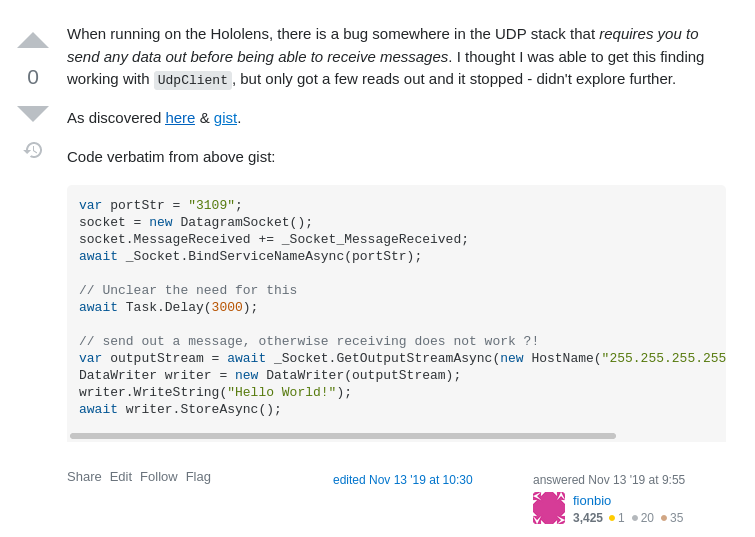
\includegraphics[width=0.8\textwidth]{uwp-udp-known-bug.png}
  \caption{A weird known bug\cite{noauthor_sockets_nodate}. \gls{UDP} sockets on the Hololens require to send data before being able to receive them. The original bug was originally reported on the MSDN forum in 2017\cite{osthege_datagramsocketmessagereceived_2017}.}\label{fig:uwp_weird_bug}
\end{figure}

\begin{figure}[p]
  \centering
  \begin{tabular}{c}
  \begin{lstlisting}[language=c]
    private void OnQRCodeUpdated(object sender, QRCodeUpdatedEventArgs args)
    {
        var data = new QRCodeData();
        data.Id = new Guid(args.Code.Id.ToString());
        data.Data = new string(args.Code.Data.ToCharArray());
        data.SpatialGraphNodeId = new Guid(args.Code.SpatialGraphNodeId.ToString());
        data.PhysicalSideLength = args.Code.PhysicalSideLength;
        _executeOnMainThreadQueue.Enqueue((EventType.UPDATED, data));
    }
    \end{lstlisting}
  \end{tabular}
  \caption{This code is executed on the QR code recognition thread and dispatches the data acquired from the QR code detection to Unity's main thread. Removing the explicit copying from the \texttt{args} parameter results in a segmentation fault on the Hololens, which shouldn't be possible in a managed language like C\#. This is likely caused by a bug in some step of the conversion from C\# to native code, but given the complexity of this process it was decided to not investigate this bug further.}\label{lst:qr_code_segfault}
\end{figure}

Nevertheless, the Hololens remains a very capable platform, and despite these problems, its integration with Unity noticeably simplifies and speeds up the development of \gls{AR} experiences.